\documentclass[Rapport/Rapport_main.tex]{subfiles}
\begin{document}
\section{Arkitektur}
I de følgende afsnit beskrives arkitekturen for CarnGo, som er baseret på bilag \textbf{Kravspecifikation} og \textbf{Analyse}. Afsnittet kan dog læses uden kendskab til den fulde dokumentation af analyse og krav. Læseren henvises til bilag \textbf{Arkitektur} for den komplette dokumentation.\\\\
For at beskrive arkitekturen af det softwareintensive system bruges 4+1 modellen. Her bruges de udvalgte User Stories til at illustrere arkitekturen, og modellen bruges til at beskrive systemet ud fra forskellige perspektiver. Til sidst i afsnittet angives kravene for databasen.  
\begin{itemize}
    \item \textbf{Logical View:} Beskriver systemets funktionalitet, som leveret til slutbrugerene. Dette illustreres vha. applikationsmodeller. Da der laves en WPF-applikation er Model-view-viewmodel(MVVM) brugt til at beskrive software arkitekturen. 
    \item \textbf{Process View:} Beskriver systemetprocesserne og hvordan de kommunikerer, samt systemets runtimeadfærd.
    \item \textbf{Deployment View:} For at beskrive systemkomponenterne anvendes et package diagram. 
    \item \textbf{Physical View:} Beskriver de fysiske lag såvel som de fysiske forbindelser mellem komponenter. Dette illustreres med et deployment diagram. 
    \item \textbf{Scenerier}: Her bruges User Stories til at illustrere arkitekturen. USDD diagrammet viser hvordan scenerierne fra User Stories bliver samlet til en helhed, for at beskrive systemets forskellige elementer og funktionalitet (se figur \ref{fig:USDD}). \\\\
    \textbf{USDD diagrammet er ikke et foruddefineret værktøj}, men et der bliver brugt til at give overblik over hvordan User Stories bliver fordelt til systemfunktionalitet i dette projekt. Det har samme aspekter som et User Story Map, hvor User Stories bliver kategoriseret under et fælles 'Epic' (overordnet tema).
    \item \textbf{Security View:} Der tilføjes også et sikkerhedsview, som fokuserer på, hvordan systemet implementeres ud fra sikkerhedsmæssige elementer, og hvordan sikkerhed påvirker systemegenskaberne. 
\end{itemize} \newpage 

\subsection{User Story Distribution Diagram}
User Story Distribution Diagrammet viser User Stories sammenhæng med arkitekturen. Views i 4+1 modellen tager udgangspunkt i distributionerne. 
\begin{figure}[H]
    \centering
    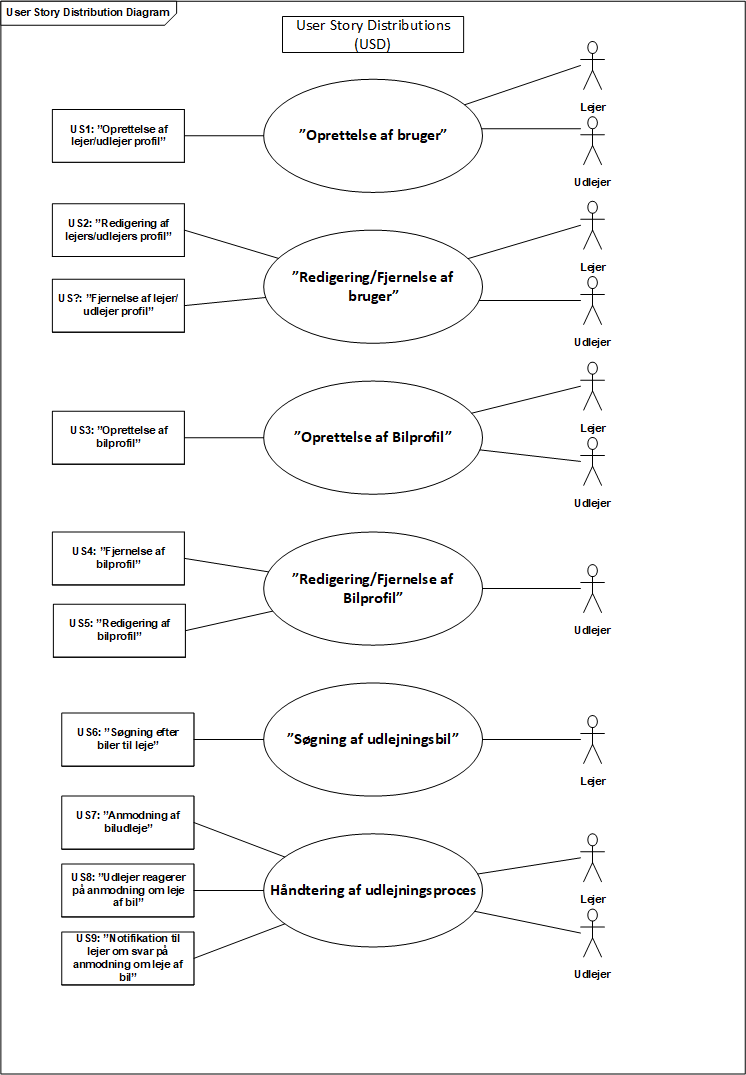
\includegraphics[width=0.90\textwidth]{Kravspecifikation/Funktionelle_krav/UserStories/graphics/USDD.png}
    \caption{User Story Distribution Diagram (USDD)}
    \label{fig:USDD}
\end{figure}
User Stories er strukturet ud fra det domæne angivet i \textbf{Problemformuleringen} og \textbf{Kravspecifikationen}. Figur \ref{fig:domain} konceptualiserer domænet og beskriver dets adfærd og data. Domænemodellen angiver systemets eksterne og interne aktører/roller, som interagerer med softwarekomponenterne. Her introduceres rollerne i systemet, og hvilke rettigheder og muligheder de har i forhold til interaktionen med systemet og dets data. Kasserne skal ses som softwarekomponenter eller koncepter for systemet. Aktørerne er de roller brugeren kan have i systemet - de er en 'User', indtil de registeres i systemet; enten som 'Renter' eller 'Lessor'. 
\begin{figure}[H]
    \centering
    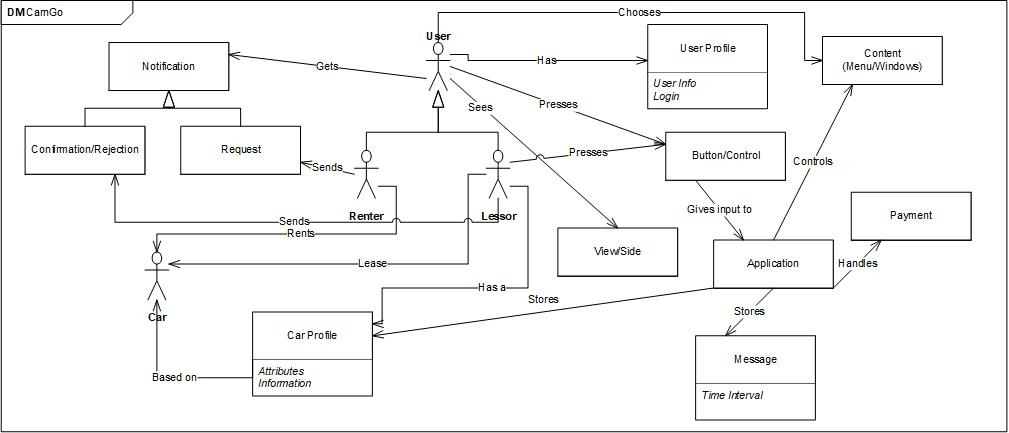
\includegraphics[width=1\textwidth]{Arkitektur/Softwarearkitektur/UserStoryArchitecture/graphics/DomainModel.jpg}
    \caption{Domænemodel af CarnGo-systemet.}
    \label{fig:domain}
\end{figure}
Wireframet nedenfor illustrerer programmets flow, og de vinduer som er konceptualiseret ud fra domænet og kravene angivet i bilag \textbf{Kravspecifikation}. Navigationen mellem de forskellige frames og deres karaktistika afspejles i applikationsmodellerne for det logiske view. 
!!!!!!!!!!!!INDSÆT WIREFRAME!!!

De næste afsnit vil gennemgå systemets arkitektur, grænseflade og adfærd. \newpage

\subfile{Rapport/Arkitektur/4+1/Scenerio/Scenerio.tex} \newpage
\subfile{Rapport/Arkitektur/4+1/Logical/Logical.tex}\newpage 
\subfile{Rapport/Arkitektur/4+1/Process/Process.tex}\newpage 
\subfile{Rapport/Arkitektur/4+1/Physical/Physical.tex}\newpage 
\subfile{Rapport/Arkitektur/4+1/Development/Development.tex}\newpage 
\subfile{Rapport/Arkitektur/4+1/Security/Security.tex} \newpage

\subsection{Database}
Databasen for CarnGo skal kunne håndtere udlejere, lejere og biler. Udlejere ejer biler, og lejere kan leje biler i bestemte tidsintervaller angivet af udlejer. \\
Biler skal være tilknyttet en udlejer, som kun kan lejes til \textbf{en} lejer ad gangen og skal kunne blive midlertidigt reserveret af lejere uden samtykke fra udlejere imens en anmodning om at leje bilen behandles. Bilen skal frigives fra midlertidigt reservering, når udlejer godkender eller afviser udlejningen. Hvis udlejningen godkendes, skal bilen markeres som udlejet i det angivne tidsinterval. Biler skal have en nummerplade, og udlejeren skal angive biltype, lokation, vægt, højde, bredde og i hvilke tidsintervaller det er muligt at leje den. Lejeren kan søge efter biler ud fra dets karakteristik og attributter (tidsinterval, biltype og lokation). \\\\
Udlejere må registrere alle de biler de ønsker, og lejere må leje så mange biler de vil. Både lejere og udlejere skal have kontaktinformation, kørekortnummer og navn. \\\\
Databasen skal understøtte et besked system, hvor lejer skriver en besked til udlejer i forhold til biludlejning i et tidsinterval. Udlejer skal kunne svare på beskeden, hvor han/hun enten kan godkende eller afvise anmodningen. Figur \ref{fig:dab} illustrerer de vigtigste elementer for databasen
\begin{figure}[H]
    \centering
    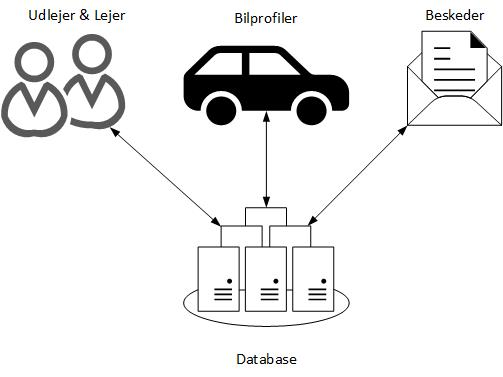
\includegraphics[width=0.8\textwidth]{Rapport/Arkitektur/4+1/Logical/graphics/DatabaseIllustration.jpg}
    \caption{Skitse af hovedelementer for CarnGo databasen}
    \label{fig:dab}
\end{figure}

\end{document}